\documentclass[11pt]{scrartcl}

\title{Anforderungsspezifikation}
\author{Silvan Adrian \\ Fabian Binna \\ Pascal Kistler}
\date{\today{}}

\usepackage[ngerman]{babel}
\usepackage[automark]{scrpage2}
\usepackage{hyperref}
\usepackage{color}
\usepackage[normalem]{ulem}
\usepackage{scrpage2}
\usepackage{graphicx}
\usepackage{tabularx}
\graphicspath{ {./images/} }
\pagestyle{scrheadings}
\usepackage{wrapfig}

\clearscrheadfoot
\ihead{
\includegraphics[scale=0.4]{jbomberman}}
\ohead{Projekt: JBomberman}
\ifoot{Anforderungsspezifikation}
\cfoot{Version: 1.00}
\ofoot{Datum: \today{}}
\setheadsepline{0.5pt}
\setfootsepline{0.5pt}

\usepackage{ucs}
\usepackage[utf8]{inputenc}
\usepackage[T1]{fontenc}


\begin{document}
\def\arraystretch{1.5}
\begin{titlepage}
\begin{center}
\vspace{10em}

\includegraphics[scale=2]{jbomberman}
\vspace{10em}
\end{center}
\begin{center}
\huge {Projekt: JBomberman} \\
\huge {Anforderungsspezifikation}
\end{center}
\begin{center}
\vspace{10em}
\LARGE {Pascal Kistler} \\
\LARGE {Silvan Adrian} \\
\LARGE {Fabian Binna}
\end{center}

\end{titlepage}

\newpage
\section{Änderungshistorie}
\label{sec:Änderungen}

\begin{tabularx}{\linewidth}{l l l l}
\textbf{Datum} & \textbf{Version} & \textbf{Änderung}  & \textbf{Autor} \\
\hline
\textbf{09.03.15} & 1.00 & Erstellung des Dokuments & Gruppe \\
\end{tabularx}

\newpage
\tableofcontents
\newpage
\section{Einführung}
\label{sec:Einführung}

\subsection{Gültigkeit}
\label{sec:Gültigkeit}

\subsection{Referenzen}
\label{sec:Referenzen}

\subsection{Übersicht}
\label{sec:Übersicht}

\section{Allgemein Beschreibung}
\label{sec:Allgemeine Beschreibung}

\subsection{Produkt Perspektive}
\label{sec:Produkt Perspektive}

\subsection{Produkt Funktion}
\label{sec:Produkt Funktion}

\subsection{Benutzer Chrakteristik}
\label{sec:Benutzer Chrakteristik}

\subsection{Einschränkungen}
\label{sec:Einschränkungen}

\subsection{Annahmen}
\label{sec:Annahmen}

\subsection{Abhängigkeit}
\label{sec:Abhängigkeit}

\section{Detailiertes Spielprinzip}
\label{sec:Detailiertes Spielprinzip}
\subsection{Allgemeine Beschreibung}
\label{Allgemeine Beschreibung}
In der klassischen Variante besteht das Spielfeld aus einer Anordnung 
von zerstörbaren und unzerstörbaren Wänden. 
Durch das Legen von Bomben können somit immer mehr 
Bereiche des Spielfelds erschlossen werden. Hinter einigen 
Wänden verstecken sich Bonusgegenstände.\cite{Bomberman Spielprinzip}

\subsection{Spielelemente}
\label{sec:Spielelemente}
\subsubsection{Statusanzeige}
\label{sec:Statusanzeige}
In der Statusanzeige wird für jeden einzelnen Bomberman (1-4 Spieler) die Anzahl 
Gewinne und ein Timer der runterzählt angezeigt.
\subsubsection{Spielfeld}
\label{sec:Spielfeld}
Das Spielfeld wird sich auf eine Grösse von ca. 13 Blöcken x 13 Blöcken 
erstrecken.
Die Wände sind dabei unzerstörbar, damit die bis zu 4 Bombermans das Spielfeld 
nicht verlassen können.
Jeder Ecken im Spielfeld ist für einen Bomberman festgelegt, bei weniger als 4 
Spielern bleiben die übrigen Ecken einfach leer.

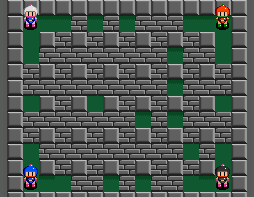
\includegraphics[scale=1.5]{bombermanmap} 

\cite{Bomberman Spielfeld}

\subsection{Wände}
\label{sec:Wände}
\subsubsection{Unzerstörbar}
\label{sec:Unzerstörbar}
\begin{table}[h]
\begin{tabularx}{\linewidth}{l X }
     
       
\includegraphics[]{solidblock}
      & Die unzerstörbaren Wände können von keiner Bombe zerstört noch von einem 
Bomberman durchlaufen werden.
\end{tabularx}
\end{table}

\subsubsection{Zerstörbar}
\label{sec:Zerstörbar}

\begin{table}[h]
  \begin{tabularx}{\textwidth}{l X }
    
    
      
\includegraphics[]{explodableblock} & Die zerstörbaren Wände können von 
    einer Bombe zerstört werden, bevor Sie zerstört sind kann ein Bomberman 
    nicht durchlaufen.
  \end{tabularx}
\end{table}

\subsection{Bomberman}
\label{subsec:Bomberman}
Der Bomberman ist der steuerbare Charakter im Bomberman Spiel, dabei kann er 
sich in alle Himmelsrichtungen bewegen.
Es sei denn ein Hindernis ist im Weg, dann kann er sicht nicht weiter bewegen.

\subsection{Bombe}
\label{subsec:Bombe}
Die Bombe ist wohl der wichtigste Gegenstand im Bomberman, denn ohne die Bombe 
könnten sich die Bombermans ihren Weg nicht freiräumen.
Somit ist die Funktion der Bombe das beseitigen von zerstörbaren Wände und um 
Gegenspieler frühzeitig aus dem Spiel zu werfen.
\subsection{Power Ups}
\label{subsec:Power Ups}
Durch zerstören, der zerstörbaren Wände kommen Power Ups zutage, welche einen 
gewissen Einfluss auf das Spielerlebnis haben.

\subsubsection{Bombe}
\label{subsubsec:Bombe}

\subsubsection{Stiefel}
\label{subsubsection:Stiefel}

\subsubsection{Flamme}
\label{subsubsection:Flamme}

\section{Use Cases}
\label{sec:Use Cases}

\subsection{Use Case Diagramm}
\label{sec:Use Case Diagramm}

\subsection{Aktoren & Stakeholders}
\label{Aktoren & Stakeholders}

\subsection{Beschreibungen Brief}
\label{sec:Beschreibungen Brief}

\subsubsection{Use Case Name}
\label{sec:Name of Use Case}

\subsection{Beschreibungen fully dressed}
\label{sec:Beschreibungen full dressed}

\subsubsection{Use Case Name}
\label{sec:Use Case Name}

\section{Weitere Anforderungen}
\label{sec:Weitere Anforderungen}

\subsection{Qualitätsmerkmale}
\label{sec:Qualitätsmermale}

\subsection{Schnittstellen}
\label{sec:Schnittstellen}

\subsection{Randbedingungen}
\label{sec:Randbedingungen}


\begin{thebibliography}{999}
\bibitem [Spielprinzip] {Bomberman Spielprinzip} 
\url{http://de.wikipedia.org/wiki/Bomberman}, Zugriff 
11.03.2015
\bibitem [Spielfeld] {Bomberman Spielfeld} 
\url{http://images1.wikia.nocookie.net/__cb20120401191543/
bomberman/images/archive/d/d0/20120401224115!SB2Usual.png} , Zugriff 11.03.15
\end{thebibliography}

\end{document}